\chapter{Исследовательская часть}

В данном разделе будут приведены примеры работы программы, а также проведен сравнительный анализ процессорного времени работы реализаций алгоритмов при различных ситуациях на основе полученных данных.

\section{Технические характеристики}

Технические характеристики устройства, на котором выполнялись замеры времени представлены далее:

\begin{itemize}
	\item операционная система Windows 11 Pro Версия 22H2 (22621.674) \cite{wind};
	\item память 16 ГБ;
	\item процессор 11th Gen Intel(R) Core(TM) i5-11400 2.59 ГГц \cite{proc}.
\end{itemize}

При тестировании компьютер был включен в сеть электропитания. Во время замеров процессорного времени устройство было нагружено только встроенными приложениями окружения, а также системой тестирования.

\section{Демонстрация работы программы}

%На рисунке \ref{img:res} представлен результат работы программы.
%\newpage
%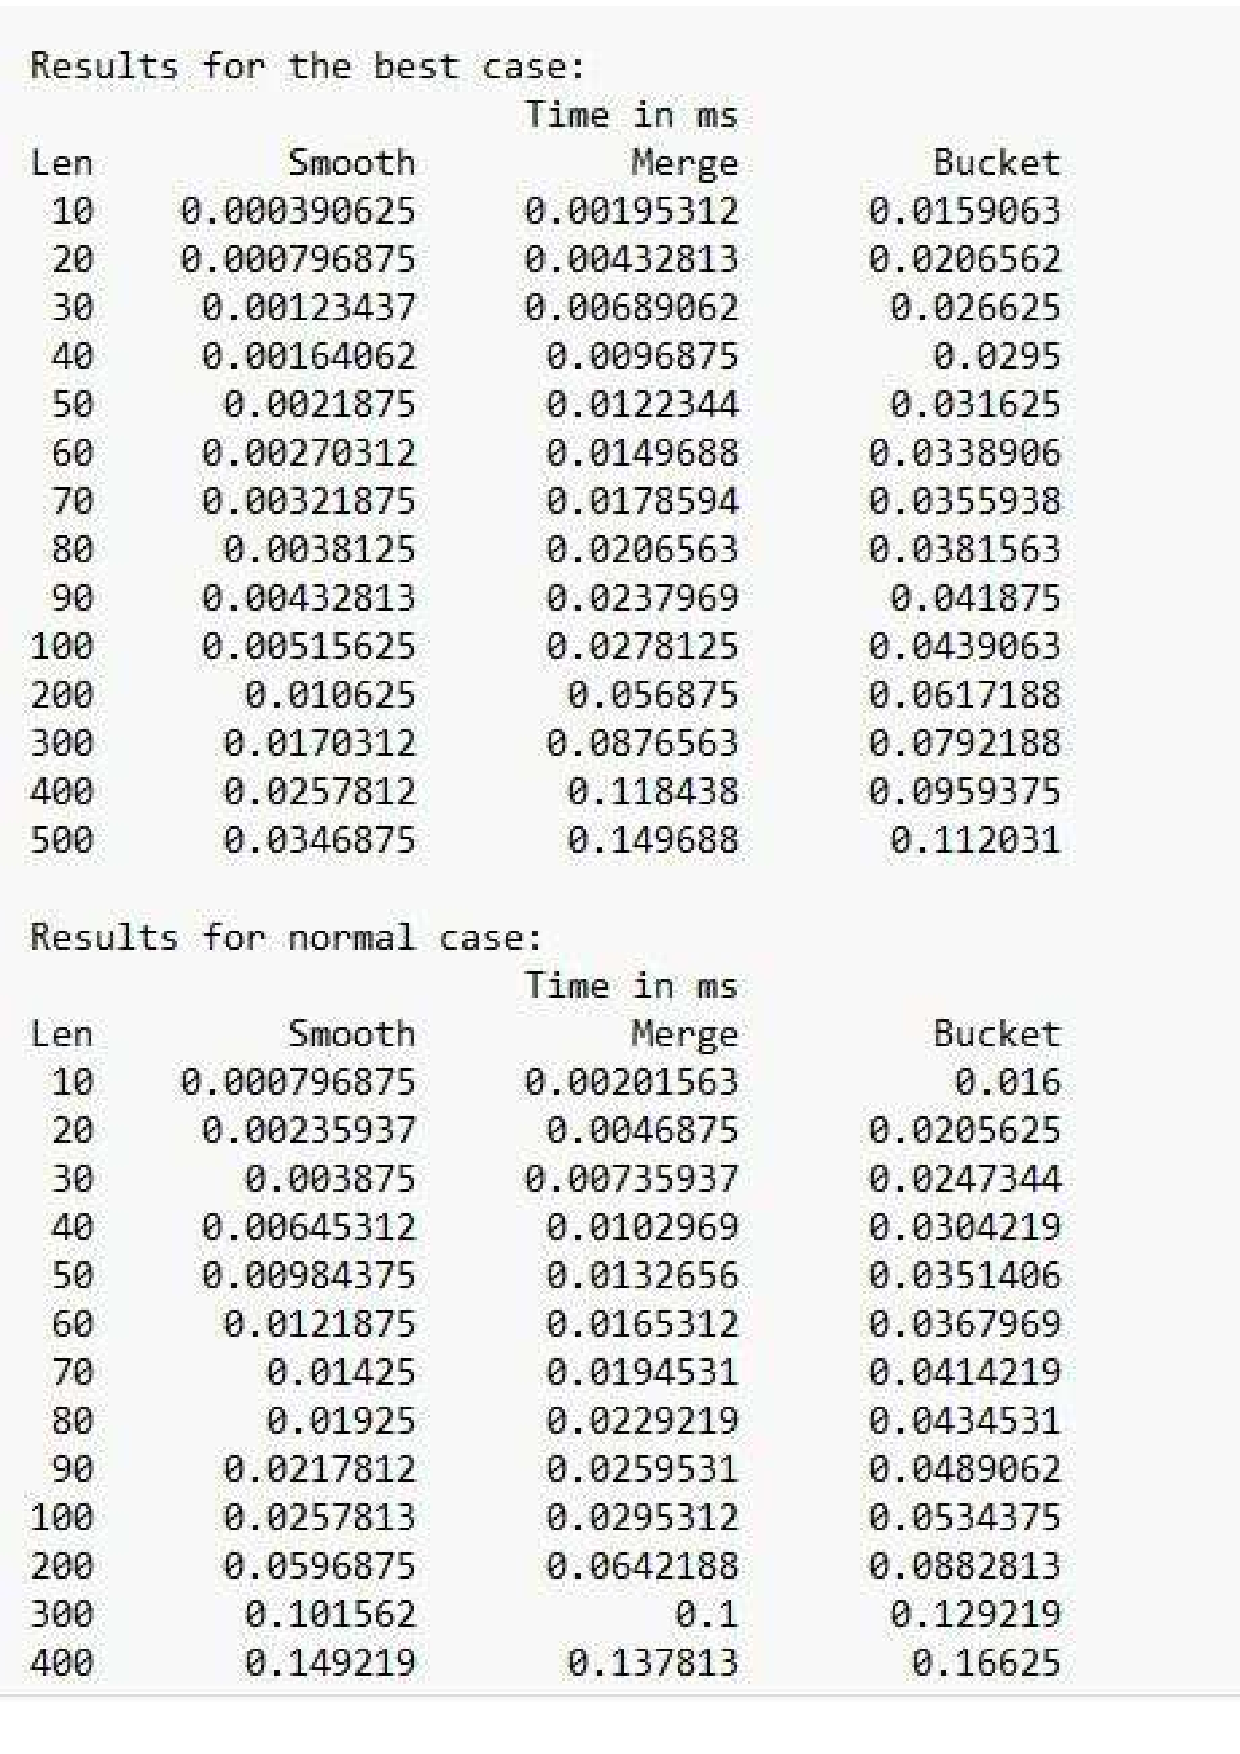
\includepdf[pages=-]{src/screen.pdf}
%\begin{center}
%	\centering{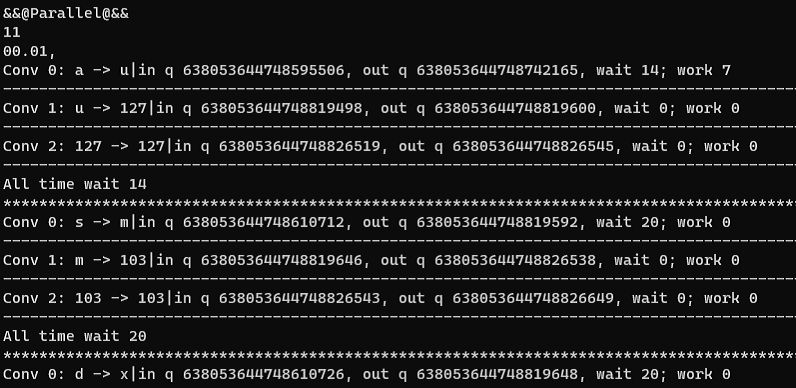
\includegraphics[trim=0 0 0cm 0cm bb=0 0 504 320]{src/screen}}
%	\captionof{figure}{Пример работы программы}
%	\label{img:res}
%\end{center}

\section{Время выполнения реализаций алгоритмов}

\textbf{Входные данные:} строки размером от 1 до 10 символов для сравнений рекурсивной версии алгоритма поиска расстояния Дамерау-Левенштейна и остальных алгоритмов; строки размером от 10 до 500 символов для остальных случаев сравнения.



\section{Вывод}
